\chapter{Background}

\section{Definitions}
\subsection{Epidemic and Pandemic }
An infectious disease is a disease that is caused by pathogenic micro organisms, such as bacteria, viruses, parasites or fungi; the diseases can be spread, directly or indirectly, from one person to another.An  epidemic is a situation where an infectious disease is affecting many people at a particular time and spread at a very high rate. A pandemic on the other is an epidemic over a large area \citep{morens2009pandemic}.

\subsection{deterministic and stochastic infectious disease models}
The dynamics of infectious disease propagation are modelled as a dynamical system. A dynamical system is a system that evolves with time over a state space according to a fixed rule. Thus, let $\mathbb{X}$ be a state space $\mathbb{T}$ set of times and $\mathbb{R}$ rule that specifies how the state evolves with time. the rule is a function  whose domain is $\mathbb{X} \times  \mathbb{T}$ and co-domain $\mathbb{X}$ that is,
\begin{equation*}
\mathbb{R}: \mathbb{X}  \times \mathbb{T} \longrightarrow \mathbb{X}.
\end{equation*}

This means that $\mathbb{R}$ takes two arguments $( \textbf{x},t)$ where $\textbf{x} \in \mathbb{X}$ is the initial state and $t \in \mathbb{T}$. That is $\mathbb{R} ( \textbf{x},t)$ give the state of the system at $t$ given the initial state of the system was $\textbf{x}$ \citep{DQ}.

The population can be characterized as $S(t)$, $E(t)$,$I(t)$ and $R(t)$ . Where $S(t)$ is the number of individuals susceptible but not infected at time $t$, $E(t)$ is the number of people exposed or infected but not infectious at time $t$, $I(t)$ is the number of infected and infectious people at time $t$ and $R(t)$ is the number of people whose  ability to be infected is removed, by either immunization, death or recovery from the disease. The epidemiological models can be classified as Susceptible,Infected and Recovered (SIR) , Susceptible Infected (SIS or SIS) , Susceptible -Exposed - Infectious and Removed (SEIR)  and by any other states the population may be partitioned into.
\Jnote{It feels to me you are contradicting yourself. If you assume
  continuous time, I don't think it is accurate to represent the disease
  evolution as ``rule'' $\mathbb{R}$.}

The SIS model assumes that there is no immunity after recovery. It is used to model infections where once a person recovers they become susceptible again.For example infections like flue. SIR model assumes that once a person recovers they become immune to the infection for example chicken pox. The SEIR assumes that once a person  becomes infected they do not  become infectious immediately hence the intermediate compartment for exposed. 


The independent variable in the compartmental model is the time $t$ .The rates of transfer between compartments are expressed mathematically as a result models are formulated initially as differential equations.Most epidemic models are built on the SIR model  \citep{m1925applications}. The system can be written as;


\begin{center}
\begin{equation} \label{eqn1_1}
\begin{array}{ccl}
\frac{dS}{dt} &= &-\alpha S(t) I(t),\\
 \frac{dI}{dt} &=& \alpha S(t) I(t) - \gamma  I(t), \\
 \frac{dR}{dt} &= &\gamma  I(t),
\end{array}  
\end{equation}
\end{center}



with assumptions that there is homogeneous mixing in the population. That is the rate of new infections is proportional to the current numbers of susceptibles and infectives in the population. Which the main assumption deterministic models are built on. Deterministic population  models are models where the behaviour of the population of determined completely by history and the rules which govern the model. In formulating these models , in terms of derivatives of the sizes of the compartments and it is assumed that the number of members in each compartment is differentiable with time. This assumption is tenable only when the disease outbreak has been established  but not valid at the beginning of a disease outbreak, when they are few infectives. When they are a few infectives, the number of infectious depends on random contacts of between small number of individuals \citep{brauer2012mathematical}.
 
 On the other hand Stochastic models are obtained by setting by adding a random variable called noise to the transmission dynamics of deterministic models.These random fluctuations may impact the evolution of the infection. Unlike deterministic model which assume homogeneous mix , an assumption which only holds in small populations. It is quiet unlikely that all people in will be equally susceptible to the disease and effective in spreading it \citep{ball1985deterministic}. A stochastic model can be further be described as a model in which the distribution of the length of the infectious period as allowed to have any distribution that can be describe by its Laplace transform \citep{addy1991generalized}.
\Jnote{This description is vague. Can you give a minimal example of a
  stochastic model?}
 
 Lets takes an SIR compartmental model, for $t > 0$, $S(t),I(t),R(t)$ is the number of individuals in susceptible, infectious and removed. $N(t)$ the total number of particles at time $t$. The poisson process, which is the underlying structure basic to the class of stochastic models and all Markov chain processes\citep{greenwood2009stochastic}. 
\Jnote{It is not clear to me what is the relation of poisson process to the
  rest. Explain better.}
The individuals enter each compartment at random times 
\Jnote{Why random times? I thought it is $t=0$?}
and the initial fixed values , $S(0)$,$I(0)$ and $R(0)$ are fixed for some $\lambda > 0$. 
\Jnote{What is $\lambda$?}
Letting $\beta$ to be the average number of  contacts an infectious person makes per unit of time that take leads to infection. The probability of a susceptible individual moving from compartment S to compartment I in the time interval $\left[ t,\triangle t \right]$ that is  S $\rightarrow S-1$ and I $\rightarrow I + 1 $ is $ \beta$ S I $ \triangle t + o (\triangle t)$. If it is assumed the an infected person recovers at the rate $\gamma$ hence the probability of an infected person moving from infected to recovered over an interval $\left[ t,\triangle t \right]$  given by $\gamma I_{t + \triangle t} -o (\triangle t)$ .It is known that,
 \begin{align*}
 N_t = S_t + I_t + R_t
 \\ \Rightarrow  R_t = N_t - S_t - I_t
\end{align*}  
Which implies that knowing $S_t,I_t$ is knowing $R_t$. Hence the model becomes an $S_t,I_t$ and thus the stochastic dynamical system can be written as;
 \begin{align}
 P((S_{t + \triangle t}, I_{t + \triangle t} - (S_t ,I_t) = ( - 1,1)) =  \beta S I  \triangle t + o (\triangle t).
 \\ P (((S_{t + \triangle t}, I_{t + \triangle t} - (S_t ,I_t) = ( 0,-1)) = \gamma I_{t + \triangle t} -o (\triangle t).
 \end{align}
 \Jnote{I think you are trying to give an example of a stochastic model,
   but I realized that only at the end of the paragraph. You should rewrite it.
   Also give more details about this model. Most important:
   is time discrete or continuouos?}
\subsection{Network}


 A graph also known as a network   can be  defined as couple $G = (V,E)$ where $V$ is a finite set of nodes $E \subset V \oplus V = \left\lbrace e_1,e_2,\dots ,e_m \right\rbrace$ is a set and f is a mapping which associates some elements of $E$ to a pair of elements of $V$ \citep{estrada2012structure}. Nodes can be human beings, cities or houses while edges could be any connection such as friendship, physical connection or road.

A network is said to be connected if there exist a path between any two nodes in the network.Distance between any two nodes in a network is defined as the length of the shortest path by which each a node can be reached. This can be summed up as the average distance taken over all pairs of vertices , which give the idea of the typical distance between nodes in a network. The diameter of the graph  is the largest distance taken over all pairs.

\subsection{Statistical Characterization}
 
 Networks can be characterized by the following statistical properties.
 \begin{itemize}
 \item[i] \textit{\textbf{Degree distribution}}
 The degree of a node is the number of connections a particular node has  and is denoted as $k$  and the average distribution of a network is denoted by $\langle k \rangle$. 

Looking at the entire space or network one can obtain a distribution for the degree. Let $n(k)$ be the number of nodes of degree $k$  in a network of size $n$, $p(k) = \dfrac{n(k)}{n}$. $p(k)$ represents the probability that a node selected uniformly at random  has degree $k$. the degree distribution is obtained by plotting $p(k)$ against $k$\citep{estrada2015first}. The common distribution found in network are normal distribution, exponential, power law distribution and poisson distribution.
   \citep{chung2002average}.
   
 \item[ii] \textit{\textbf{Clustering }}
 A cluster in a network  is a collection of nodes which are similar among them and are dissimilar to other nodes belonging to other clusters. Clustering in friendship network may mean friends people have in common. Local clustering in a network is measured by   the Watts -stoggatz  coefficient and the global clustering by  Newman clustering coefficients.
 
 Watts -strogatz average clustering coefficient is given by 
 \begin{align}
 \overline{C} = \dfrac{1}{n} \sum_i c_i
  \\ c_i = \dfrac{2t_i}{k_i(k_i-1)} \nonumber
  \end{align}
   where $t_i $ the  number of triangles attached to node $i$ of degree $k_i$. The Watts-Strogatz clustering coefficient of a node quantifies how close its neighbours are close to making a clique. In terms of friends it quantifies how ones friends are friends with each other. The clustering coefficient  lies between 0 and 1, if it zero then node of a nodes neighbours are connected and  if it is 1 then then all the neighbours of a node are connected to connected to each other.
  

 The Newman clustering coefficient is given by
 \begin{equation}
 c = \frac{3t}{p_2} =\dfrac{3|c_3|}{p_2}
 \end{equation}
 where $t = c_3$ number of triangle in the network and $|p_2|$ the number of closed paths of length 2. 
\end{itemize}

 The Newman clustering coefficient or so know as the network clustering coefficient, gives the average clustering for the whole network. Node with less than two neighbours are given 0 as the clustering coefficient. It looks at the clustering over the whole network.
 
 In a social network if a person A is friends with person B and B friends with C most likely A will be introduced to C and the two will know each other. This will result in the three forming a triangle. The clustering coefficient either global or local gives a proportion of how many such triangles are there and how many are likely to exist. The local will give this value in relation to a particular node while the global will give the value over the entire  network \citep{estrada2015first}.
 
 A network is said to be small world or to exhibit small world properties if its Newman clustering coefficient is greater than the Watts- strogatz clustering coefficient. That is a small world network has a high clustering coefficient and low average distance \citep{estrada2012structure}. A small world property can be defined as let $D$ be the average distance between any pair of vertices in a network, if $D$ increase proportionally to the logarithm of the size of the network$N$ \citep{newman1999scaling}.That is,
 \begin{equation}
 D \propto \log N
 \end{equation}
 
\subsection{Random Graphs} 
 A random graph $G(n,p)$ can be defined as , given  $N$ number of vertices, edges between them are drown such that between any pair $i,j$ there is an edge with uncorrelated probability $p$. 

Taking $z$ to be the average degree. The probability p of and edge being present between any two vertices is given by $p = \frac{z}{n-1}$, for large n can be approximated  $\frac{z}{n}$  \citep{newman2002random}. The number of nodes connected to any particular vertex, the degree $k$ of that vertex has a probability distribution $p_k$ given by;
 \begin{equation}
 p_k = \binom{n}{k} p^k (1-p)^{n-k} \approx \frac{z^k e^{-z}}{k!}.
 \end{equation}
   For example let us take 20 vertices draw and edge between with probability $p = 0.2$ We can get a random network presented in \ref{fig:3.1} below. A random network model can exhibit the small world network property. 
   It can be shown that a random graph can exhibit small world effects. Assuming that person A, represents a node on network such as  figure \ref{fig:3.1}. A has $z$ neighbours and  about $z^2$ , $z^3$  second and third neighbours respectively, and so on. Then the diameter of the network $D$ is given by $z^D = n$. Thus
   \begin{equation*}
   D = \frac{\log n}{\log z}
   \end{equation*}
    The logarithmic increase in the diameter of the network and the distance between node is typical of a small world effect. Since $\log n$ increases slowly with $n$ it allows the distance to be quite small in very large systems \citep{newman2000models}.
    A random graph  has an average degree $z= pN$. Random networks have a low clustering coefficient $ c = \frac{z}{N}$ \citep{newman2003structure}.
   \begin{figure}[h!]
   \caption{Random Graph with n =20 and p = 0.2}
   \label{fig:3.1}
   \centering
   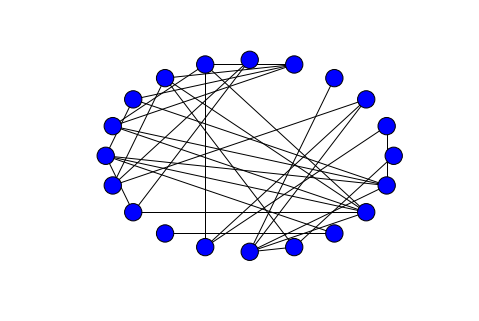
\includegraphics[scale=0.5]{images/randomgraph.png} 
   \end{figure}
   
%
%
%\begin{figure}[h]
%    \centering
%    \begin{subfigure}[b]{0.3\textwidth}
%        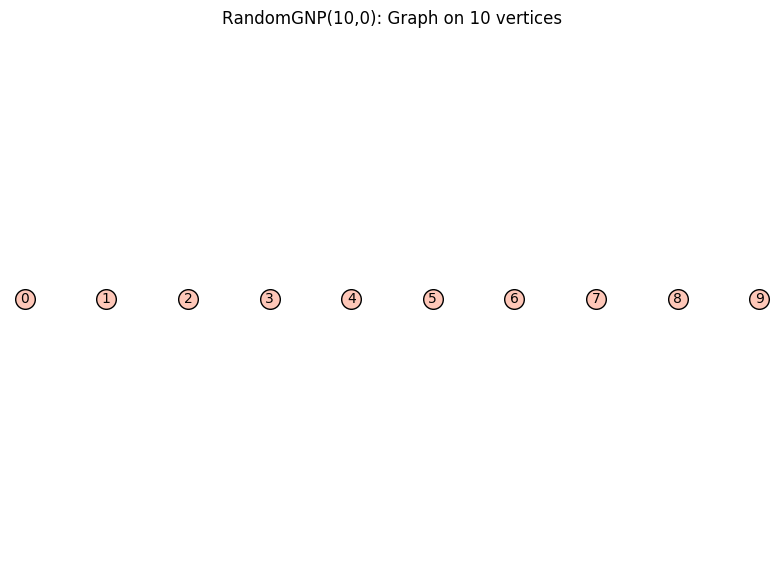
\includegraphics[scale=0.3]{images/rgraph2.png} 
%        \caption{ $p =0$}
%        \label{fig:a}
%    \end{subfigure}
%    ~ %add desired spacing between images, e. g. ~, \quad, \qquad, \hfill etc. 
%      %(or a blank line to force the subfigure onto a new line)
%    \begin{subfigure}[b]{0.3\textwidth}
%        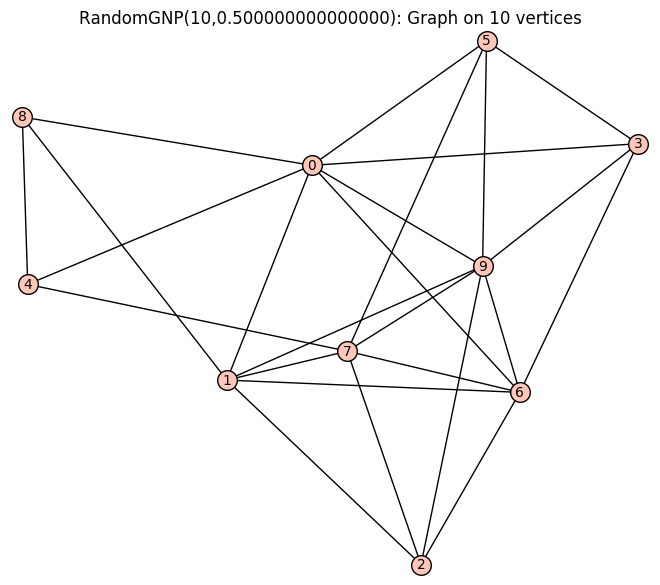
\includegraphics[width=\textwidth]{images/rgraph1.png}
%        \caption{$p=0.5$}
%        \label{fig:b}
%    \end{subfigure}
%    ~ %add desired spacing between images, e. g. ~, \quad, \qquad, \hfill etc. 
%    %(or a blank line to force the subfigure onto a new line)
%    \begin{subfigure}[b]{0.3\textwidth}
%        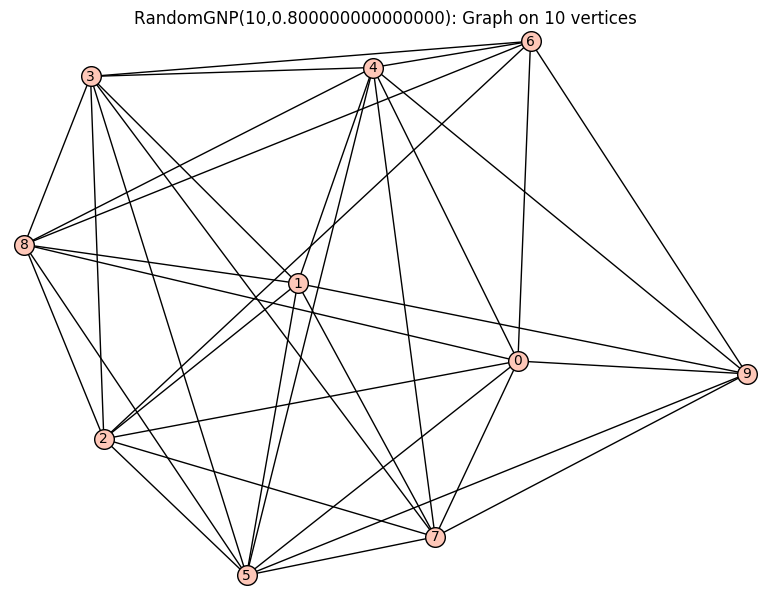
\includegraphics[width=\textwidth]{images/rgraph3}
%        \caption{$p= 0.8$}
%        \label{fig:c}
%    \end{subfigure}
%    \caption{Random Graphs}\label{fig:randomgraphs}
%\end{figure}
%
However,  random  networks  are  not  a  good  model  of  social  networks.  People’s  circles  of  
acquaintances  tend  to  overlap  to  a  great  extent. Random models have a very low clustering coefficient.
\subsection{Odered Lattice}
In order to deal with real work networks, graphs mus have both clustering and small work effect property. Random graphs as discussed earlier show a small work effect. The average vertex to vertex distances increase only logarithmically with n but does not show clustering \citep{newman2000models}. This leads us to another graph model which is an ordered lattice.

The opposite of a random graph is a completely ordered lattice. An ordered lattice is a graph where each vertex is connected to its $z$ neighbours. A lattice can be drawn in many dimensions. For example figure \ref{fig2222} shows two lattices drawn in different dimensions.
\begin{figure}[h!]
    \centering
    \begin{subfigure}[b]{0.4\textwidth}
        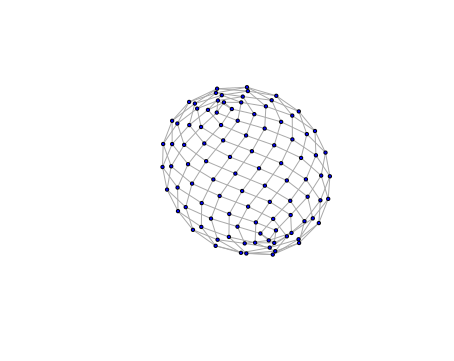
\includegraphics[scale=0.6]{images/lattice1.png} 
        \caption{A square lattice, with $z$ =4}
        \label{fig:gull}
    \end{subfigure}
    ~ %add desired spacing between images, e. g. ~, \quad, \qquad, \hfill etc. 
      %(or a blank line to force the subfigure onto a new line)
    \begin{subfigure}[b]{0.4\textwidth}
        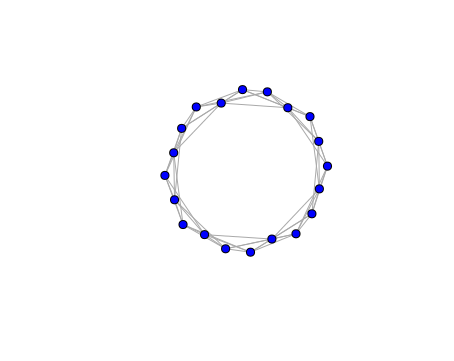
\includegraphics[scale=0.6]{images/ringlattice.png} 
        \caption{A ring lattice, with $z$ = 3}
        \label{fig ring}
    \end{subfigure}
    ~ %add desired spacing between images, e. g. ~, \quad, \qquad, \hfill etc. 
    %(or a blank line to force the subfigure onto a new line)
    \caption{Different types of regular lattices}\label{fig2222}
\end{figure}


Regular lattices and random graphs have a long history of use in network theory and to model population structures,  gives an example of classic lattice \citep{harris1974contact}.

The clustering coefficient for a lattice is given as  
\begin{equation}
C = \frac{3(z -d)}{4(2-z)}
\end{equation}
where $d$ is the dimension of the lattice.

However, regular lattices do not show the small world effect of vertex to vertex distances which increase slowly with size. For a regular lattice of dimensions with the shape of a square or hypercube of size L with $n = L^d$ vertices, the average vertex to vertex distance increases linearly with the system size, which is not typical to the small world behaviour. 


 Models built on latices assume that individuals are located as nodes on a regular lattice and connections are made of some collection of near neighbours or each node. For example people may be spread out such that connections are made to their four nearest neighbours, one on the left,right, up and down this is called a Neumann neighbours  or eight neighbours where four diagonal elements are added to the Neuman neighbours and this is called the Moore neighbour hood \citep{lloyd2006infection}.To avoid the effect of the nodes at the end not being connected the last and first neighbours are made neighbours.

The main difference between a random graph and lattices is that interactions are local, that is individuals are only related to their neighbours. Where as in random networks the connections are made are global, that is connections are made without taking spatial locations of an individual into consideration. 

\subsection{Watts - Strogats Small World Networks}
We have shown that lattices are characterised by high clustering coefficients but long path lengths or vertex to vertex distances. That is it takes many steps to move between any two randomly selected vertices, where as random networks have shorter vertex to vertex distances, since there are many long range links, but low clustering \citep{keeling2005networks}.


Small world networks  were first introduced by Watts and Strogatz as an intermediate between the regular lattice and randomly rewiring certain proportions $p$ of the network links\citep{watts1998collective}. The small world networks allows for random contacts across the network. That is in addition to near neighbours as in a regular lattice, each node has a random distant neighbour connected to it \citep{watts1998collective}.


The Watts-Strogatz network is essentially a regular lattice with some degree of randomness in the connectivity of vertices. Take for example figure \ref{fig ring} above and we rewire some edges with a some probability $p$, that is one of its ends is moved into a randomly chosen position in the lattice. For a small $p$ this produces mostly a regular graph but with a few connections stretch along distances across the lattice and for $p 1$ it produced a complete graph. Figure \ref below shows Watts- Strogats networks with different probabilities.

\begin{figure}[h!]
    \centering
    \begin{subfigure}[b]{0.4\textwidth}
        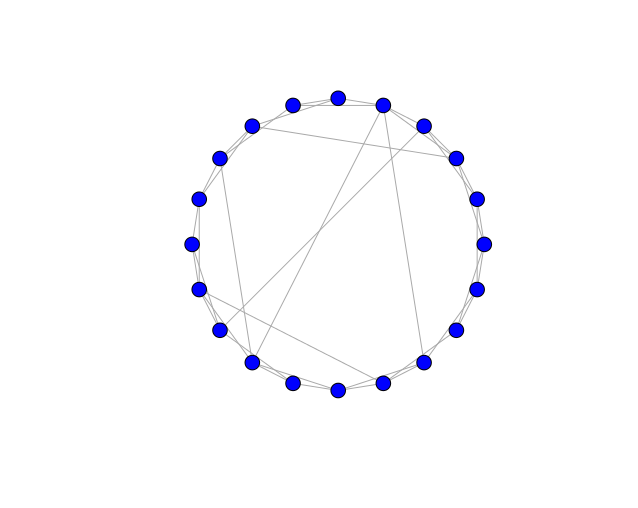
\includegraphics[scale=0.4]{images/sw_p1.png} 
        \caption{A Small world, with $p$ =4}
        \label{fig:gull}
    \end{subfigure}
    ~ %add desired spacing between images, e. g. ~, \quad, \qquad, \hfill etc. 
      %(or a blank line to force the subfigure onto a new line)
    \begin{subfigure}[b]{0.4\textwidth}
        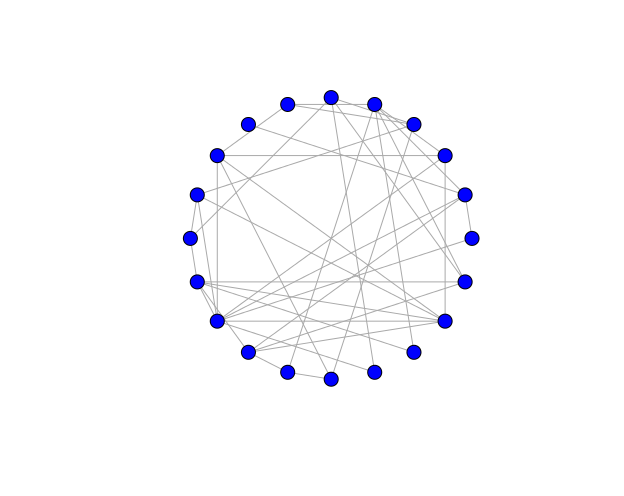
\includegraphics[scale=0.4]{images/sw_p5.png} 
        \caption{A Small world network, with $p$ = 0.5}
        \label{fig }
    \end{subfigure}
    ~ %add desired spacing between images, e. g. ~, \quad, \qquad, \hfill etc. 
    %(or a blank line to force the subfigure onto a new line)
    \begin{subfigure}[b]{0.4\textwidth}
        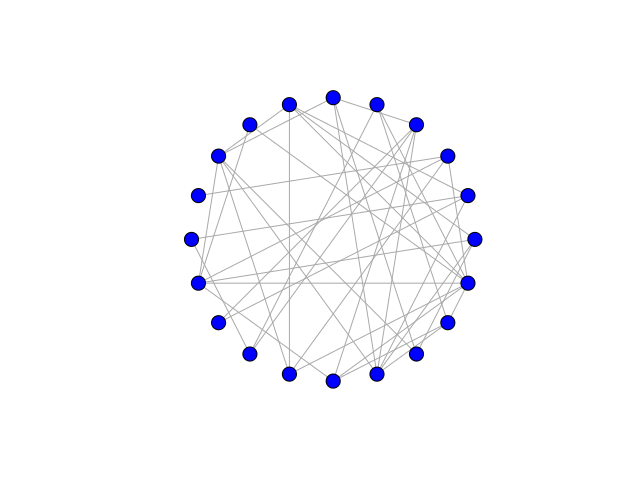
\includegraphics[scale=0.4]{images/sw_p8.png} 
        \caption{A Small world network, with $p$ = 0.8}
        \label{fig }
    \end{subfigure}
    \caption{Watts- Strogatz}\label{fig networks}
\end{figure}

 
  